\documentclass[conference]{IEEEtran}
\IEEEoverridecommandlockouts
% The preceding line is only needed to identify funding in the first footnote. If that is unneeded, please comment it out.
\usepackage{cite}
\usepackage{amsmath,amssymb,amsfonts}
\usepackage{algorithmic}
\usepackage{graphicx}
\usepackage{textcomp}
\usepackage{xcolor}
\def\BibTeX{{\rm B\kern-.05em{\sc i\kern-.025em b}\kern-.08em
    T\kern-.1667em\lower.7ex\hbox{E}\kern-.125emX}}
\begin{document}

\title{Conference Paper Title*\\
{\footnotesize \textsuperscript{*}Note: Sub-titles are not captured in Xplore and
should not be used}
\thanks{Identify applicable funding agency here. If none, delete this.}
}

\author{\IEEEauthorblockN{1\textsuperscript{st} Given Name Surname}
\IEEEauthorblockA{\textit{dept. name of organization (of Aff.)} \\
\textit{name of organization (of Aff.)}\\
City, Country \\
email address or ORCID}





}

\maketitle





\section{Project}
A smart home system has many features that can make life easier. For example, consider a smart heating and cooling system in which the heater and air conditioner can be easily adjusted via smartphone. A smart door, smart alarm, and smart light system are also examples of smart house systems. However, in our project, we will only demonstrate how the smart light system works in the smart home system.


\subsection{Hardware}

A lot of hardware is required for our project. Each piece of hardware will serve a specific purpose in the creation of our project. The list of hardware required for our projects, as well as a description of its function in our project, is provided below.


\subsection{Features and List of commands}
The smartphone in our smart light system will communicate with the server via BLE protocol to control the features that have been implemented in our smart light system. Our smart lighting system's features are listed below. Some commands have been specified and inserted on the smartphone that is already connected to the ESP32 via BLE in order for our features to show their output. It means that different commands will produce different results. In addition, users must download specific apps, which will assist in connecting to EPS32 and inserting commands. Figure 1 depicts the apps we used to connect our smartphone to the ESP32. If you have an iPhone, you can easily find this app in the "Apple store." Figure 3 also shows where the command must be inserted in order to produce the desired output.




\begin{table}[]
\caption{List of hardware and its function}
\begin{center}
\begin{tabular}{|l|l|}
\hline
Hardware                                                                   & Functions                                                                                                                                                                  \\ \hline
\begin{tabular}[c]{@{}l@{}}LED   (red, blue\\ , green, white)\end{tabular} & \begin{tabular}[c]{@{}l@{}}1. Indicate turn off and turn on\\ 2. Indicate brightness\\ 3. Indicate blinking\\ 4. Indicate night mode\\ 5. Indicate event lamp\end{tabular} \\ \hline
Jumper wire                                                                & \begin{tabular}[c]{@{}l@{}}1. Connect between breadboard \\     and component\end{tabular}                                                                                 \\ \hline
ESP32                                                                      & \begin{tabular}[c]{@{}l@{}}1. Support BLE protocol\\ 2. Act as a server to communicate\\     with mobile phone\end{tabular}                                                \\ \hline
USB cable                                                                  & \begin{tabular}[c]{@{}l@{}}1. Connect between ESP32 and \\ laptop to upload the code\\ 2. Support transmission and receiving data\end{tabular}                             \\ \hline
Breadboard                                                                 & 1. Place to put the components                                                                                                                                             \\ \hline
Buzzer                                                                     & 1. Play sound                                                                                                                                                              \\ \hline
Resistor 100 ohm                                                           & 1. Act as resistance                                                                                                                                                       \\ \hline
\end{tabular}
\end{center}
\end{table}




\begin{figure}[htbp]
\centerline{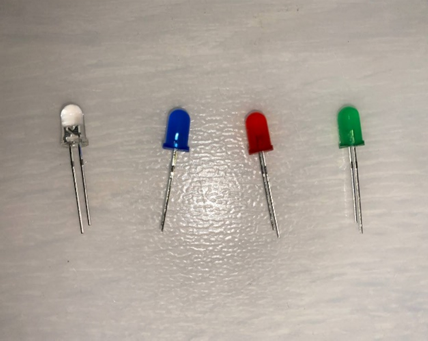
\includegraphics{image1.png}}
\caption{LED}
\label{fig}
\end{figure}

\begin{figure}[htbp]
\centerline{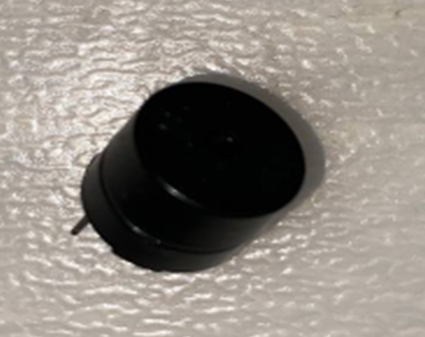
\includegraphics{image2.png}}
\caption{LED}
\label{fig}
\end{figure}

\begin{figure}[htbp]
\centerline{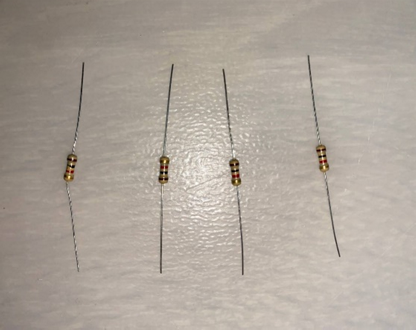
\includegraphics{image3.png}}
\caption{LED}
\label{fig}
\end{figure}

\begin{figure}[htbp]
\centerline{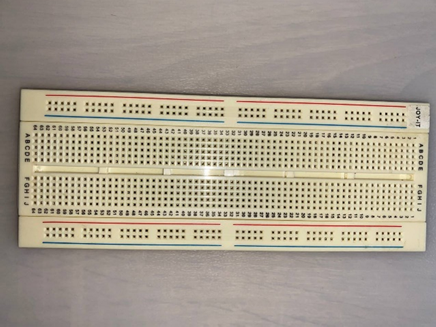
\includegraphics{image4.png}}
\caption{LED}
\label{fig}
\end{figure}

\begin{figure}[htbp]
\centerline{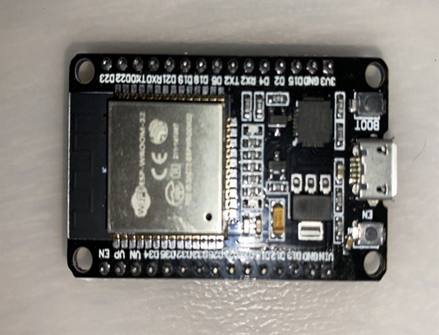
\includegraphics{image5.png}}
\caption{LED}
\label{fig}
\end{figure}





\begin{table}[]
\begin{center}
\caption{Features in Smart Light}
\begin{tabular}{|l|l|}
\hline
No & Smart   Light Features \\ \hline
2. & Turn on LED            \\ \hline
3. & Turn off LED           \\ \hline
4. & Turn on night mode     \\ \hline
5. & Turn on party mode     \\ \hline
6. & Change color           \\ \hline
7. & Play sound             \\ \hline
\end{tabular}
\end{center}
\end{table}






\begin{table}[]
\begin{center}
\caption{Lists of commands}
\begin{tabular}{|l|l|}
\hline
List of Commands & Function             \\ \hline
ONW              & Turn on white LED    \\ \hline
ONR              & Turn on red LED      \\ \hline
ONB              & Turn on blue LED     \\ \hline
ONG              & Turn on green LED    \\ \hline
OFFW             & Turn off white LED   \\ \hline
OFFR             & Turn off red LED     \\ \hline
OFFB             & Turn off blue LED    \\ \hline
OFFG             & Turn off green LED   \\ \hline
BLW              & Blinking white LED   \\ \hline
BLR              & Blinking red LED     \\ \hline
BLB              & Blinking blue LED    \\ \hline
BLG              & Blinking green LED   \\ \hline
NMW              & Night mode white LED \\ \hline
NMR              & Night mode red LED   \\ \hline
NMB              & Night mode blue LED  \\ \hline
NMG              & Night mode green LED \\ \hline
PARTY            & Party mode           \\ \hline
\end{tabular}
\end{center}
\end{table}


\begin{figure}[htbp]
\centerline{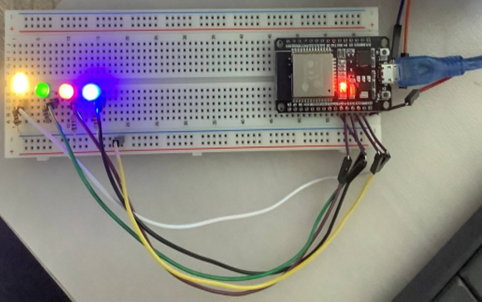
\includegraphics{image7.png}}
\caption{LED}
\label{fig}
\end{figure}




\begin{figure}[htbp]
\centerline{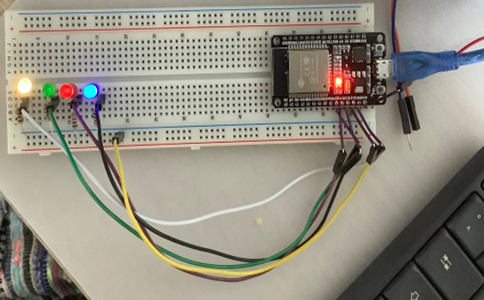
\includegraphics{image8.png}}
\caption{LED}
\label{fig}
\end{figure}


\begin{figure}[htbp]
\centerline{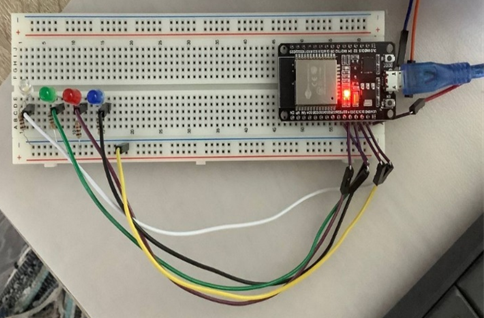
\includegraphics{image9.png}}
\caption{LED}
\label{fig}
\end{figure}



\begin{figure}[htbp]
\centerline{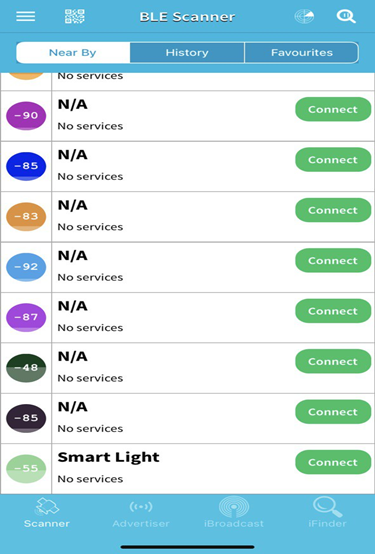
\includegraphics{image10.png}}
\caption{LED}
\label{fig}
\end{figure}




\begin{figure}[htbp]
\centerline{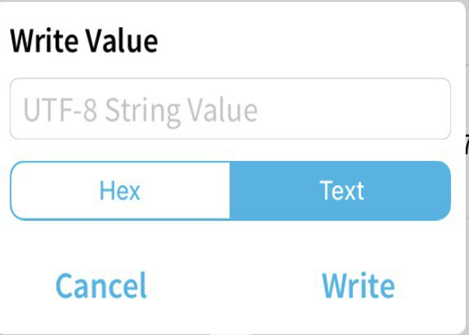
\includegraphics{image11.png}}
\caption{LED}
\label{fig}
\end{figure}








\end{document}